%%%%%%%%%%%%%%%%%%%%%%%%%%%%%%%%%%%%%%%%%
% University Assignment Title Page 
% LaTeX Template
% Version 1.0 (27/12/12)
%
% This template has been downloaded from:
% http://www.LaTeXTemplates.com
%
% Original author:
% WikiBooks (http://en.wikibooks.org/wiki/LaTeX/Title_Creation)
%
% License:
% CC BY-NC-SA 3.0 (http://creativecommons.org/licenses/by-nc-sa/3.0/)
% 
% Instructions for using this template:
% This title page is capable of being compiled as is. This is not useful for 
% including it in another document. To do this, you have two options: 
%
% 1) Copy/paste everything between \begin{document} and \end{document} 
% starting at \begin{titlepage} and paste this into another LaTeX file where you 
% want your title page.
% OR
% 2) Remove everything outside the \begin{titlepage} and \end{titlepage} and 
% move this file to the same directory as the LaTeX file you wish to add it to. 
% Then add \input{./title_page_1.tex} to your LaTeX file where you want your
% title page.
%
%%%%%%%%%%%%%%%%%%%%%%%%%%%%%%%%%%%%%%%%%
%\title{Title page with logo}
%----------------------------------------------------------------------------------------
%   PACKAGES AND OTHER DOCUMENT CONFIGURATIONS
%----------------------------------------------------------------------------------------

\documentclass[12pt]{article}
\usepackage[english]{babel}
\usepackage[utf8x]{inputenc}
\usepackage{amsmath}
\usepackage{graphicx}
\usepackage[colorinlistoftodos]{todonotes}
\usepackage{setspace}

\usepackage{amssymb}
\usepackage{enumerate}
\usepackage[english]{babel}
\usepackage{caption}
\usepackage{hyperref}
\usepackage{listings}
\usepackage{color}
\usepackage[left=1.5cm, right=1.5cm, top=1.5cm, bottom=2cm]{geometry}
\usepackage{float}
\usepackage{subcaption}
\usepackage[toc,page]{appendix}
\setlength\parindent{0pt}
\usepackage{subcaption}
\usepackage{textcomp}
\usepackage{etoolbox,refcount}
\usepackage{multicol}

\newcounter{countitems}
\newcounter{nextitemizecount}
\newcommand{\setupcountitems}{%
	\stepcounter{nextitemizecount}%
	\setcounter{countitems}{0}%
	\preto\item{\stepcounter{countitems}}%
}
\makeatletter
\newcommand{\computecountitems}{%
	\edef\@currentlabel{\number\c@countitems}%
	\label{countitems@\number\numexpr\value{nextitemizecount}-1\relax}%
}
\newcommand{\nextitemizecount}{%
	\getrefnumber{countitems@\number\c@nextitemizecount}%
}
\newcommand{\previtemizecount}{%
	\getrefnumber{countitems@\number\numexpr\value{nextitemizecount}-1x\relax}%
}
\makeatother    
\newenvironment{AutoMultiColItemize}{%
	\ifnumcomp{\nextitemizecount}{>}{3}{\begin{multicols}{2}}{}%
		\setupcountitems\begin{itemize}}%
		{\end{itemize}%
		\unskip\computecountitems\ifnumcomp{\previtemizecount}{>}{3}{\end{multicols}}{}}


\bibliographystyle{ieeetr}  

\definecolor{codegreen}{rgb}{0,0.6,0}
\definecolor{codegray}{rgb}{0.5,0.5,0.5}
\definecolor{codepurple}{rgb}{0.58,0,0.82}
\definecolor{backcolour}{rgb}{0.95,0.95,0.92}

\lstdefinestyle{mystyle}{
	backgroundcolor=\color{backcolour},   
	commentstyle=\color{codegreen},
	keywordstyle=\color{magenta},
	numberstyle=\tiny\color{codegray},
	stringstyle=\color{codepurple},
	basicstyle=\footnotesize,
	breakatwhitespace=false,         
	breaklines=true,                 
	captionpos=b,                    
	keepspaces=true,                 
	numbers=left,                    
	numbersep=5pt,                  
	showspaces=false,                
	showstringspaces=false,
	showtabs=false,                  
	tabsize=2
}

\lstset{style=mystyle}

\begin{document}
	
\doublespacing

\begin{titlepage}

\newcommand{\HRule}{\rule{\linewidth}{0.5mm}} % Defines a new command for the horizontal lines, change thickness here

\center % Center everything on the page
 
%----------------------------------------------------------------------------------------
%   HEADING SECTIONS
%----------------------------------------------------------------------------------------

\textsc{\LARGE University of Melbourne}\\[1.5cm] % Name of your university/college
\textsc{\Large SWEN90004}\\[0.5cm] % Major heading such as course name
\textsc{\large Modelling Complex Software Systems}\\[0.5cm] % Minor heading such as course title

%----------------------------------------------------------------------------------------
%   TITLE SECTION
%----------------------------------------------------------------------------------------

\HRule \\[0.4cm]
{ \huge \bfseries Wealth Distribution System}\\[0.4cm] % Title of your document
\HRule \\[1.5cm]

%----------------------------------------------------------------------------------------
%   AUTHOR SECTION
%----------------------------------------------------------------------------------------

\begin{minipage}{0.4\textwidth}
	\centering
	\bfseries     Yang Zhang(956835)\\
	\bfseries     Weikai Zeng(893814) \\
	\bfseries     Rui Zhao(860411)\\
\end{minipage}\\[2cm]

% If you don't want a supervisor, uncomment the two lines below and remove the section above
%\Large \emph{Author:}\\
%John \textsc{Smith}\\[3cm] % Your name

%----------------------------------------------------------------------------------------
%   DATE SECTION
%----------------------------------------------------------------------------------------

{\large \today}\\[2cm] % Date, change the \today to a set date if you want to be precise

%----------------------------------------------------------------------------------------
%   LOGO SECTION
%----------------------------------------------------------------------------------------


\includegraphics[scale = 0.27]{logo.png}\\[1cm] % Include a department/university logo - this will require the graphicx package
 \textsc{Word Count: 1399}\\[1.5cm]
%----------------------------------------------------------------------------------------
\vfill % Fill the rest of the page with whitespace

\end{titlepage}


\section{Background}
The Wealthy Distribution model is a complex model with a set of things working together as parts of an interconnecting network. This model has three basic objects: the world, people and grains. The world is a field with many grids. The grain grows in grids with a grown period. Each individual will gain random grains when they born and consume grains to keep alive. They keep looking for grains around the world. People have a life expectancy and they would die if they run out their grains or life.\\

As the wealth is related to everyone’s daily life, Most of the people are desired to get more wealth or resource, especially for the people who do not have sufficient resources, they dream to change their life through their effort. This model may give us some inspiration for wealthy distribution.\\

We aim to accomplish two parts\footnote{Total word count in this report: 1399}. We will concentrate on replicating the original model provided by NetLogo at first, and figure out how the properties below influence the Gini Index.
	grain growth interva,max of metabolism, number of grain grow,percentage of best land, max vision

Then, We will add three new properties, \textbf{Heritage inheritance}, \textbf{Season} and \textbf{Reclamation}, and research how these properties change the original result.
\section{Design}
\subsection{Original Model}
The domain diagram of our model is shown as below. The WorldExtension is extends from World and PeopleExtension extends from People as well.\\
%  [image]
We use a 2-dimension matrix to represent the world. Each element is a land and its value represent the grains at here. We use another matrix which has the same shape to decide the maximum capacity of lands. Thus we do not need to create a land object. Using matrix can also speed up the computing.\\
\\
There are two behaviors for a person in every clock. Firstly, everyone tries to find a best land within vision and cost some grains. When someone's age is larger than expected life expectancy, he will die and rebirth with random values of properties.
\subsection{Extensions}
Based on original model, we are going to improve its complexity by adding multiple extensions. Here we list the extensions we added in this project. 
\begin{enumerate}
	\item Heritage inheritance\\
	In original model, people will discard all the money when they are dead. In our extension, we introduce inheritance function for collecting their money when they reborn. Based on our assumption, it should be a way to speed up model development. 
	\item Season\\
	The richness of land is fixed when the world is initialized in original model. In our extended model, the richness of land varies based on different clock. We assume there are two seasons, land generates the same amount of grain as before in summer. In winter, land only generates half grain. We will find out the relationship between seasons and wealth distribution.
	\item Reclamation\\
	There should be lots of factors to impact a small part of land's richness. In order to simulate this situation, we introduce the reclamation function, which aims to improve or reduce a small part of land's richness suddenly in a time interval. We want to figure out if sudden incident will impact final wealth distribution.
\end{enumerate}
\section{Results \& Discussion}
\subsection{Pre-analyzing}
Before we run the detaild experiment of our model, we try to choose a set of hyperparameters to make the gini index change linearly. We create two index to explain the transformation of variables.\\
$$
Resource = \frac {\text {num grain grown}}{\text{grain grow interval}} * \text{percent best land} 
$$
The value of $Resource$ represent the richness of resource. The bigger the $Resource$, the easier for people to get grains.
$$
Talent = \frac {\text{max vision}}{\text{metabolism max}}
$$
The value of $Talent$ represent the ability of a people, The bigger the value, the stronger the individual.
\subsection{Results of Original Model}
According to the analysis above, we adjust the variables to increase the $Resource$ at first and then the $Talent$. Then we got 77 groups of parameters.
\begin{table}[H]
	\begin{tabular}{|c|c|c|c|c|c|}
		\hline
		Id&\#Grain Grow&Grain Grow Interval&Best Land Percentage&Max vision&Metabolism Max\\\hline
		1&1&10&5\%&1&25\\\hline
		&\vdots&&&&\\\hline
		10&10&10&5\%&1&25\\\hline
		&&\vdots&&&\\\hline
		19&10&1&5\%&1&25\\\hline
		&&&\vdots&&\\\hline
		39&10&1&25\%&1&25\\\hline
		&&&&\vdots&\\\hline
		53&10&1&25\%&15&25\\\hline
		&&&&&\vdots\\\hline
		77&10&1&25\%&15&1\\\hline
	\end{tabular}
\end{table}
Each group of parameters will run 10 times and each time will calculate the average of last 200 tickets' Gini index. Then we will calculate the average result of 10 times as the gini index of this group of parameters.\\

We use a line chart to show the result of our model. It can easily to find that the transformation of gini index is similar to the value of $Resource/Talent$.
\begin{figure}
	\begin{center}
		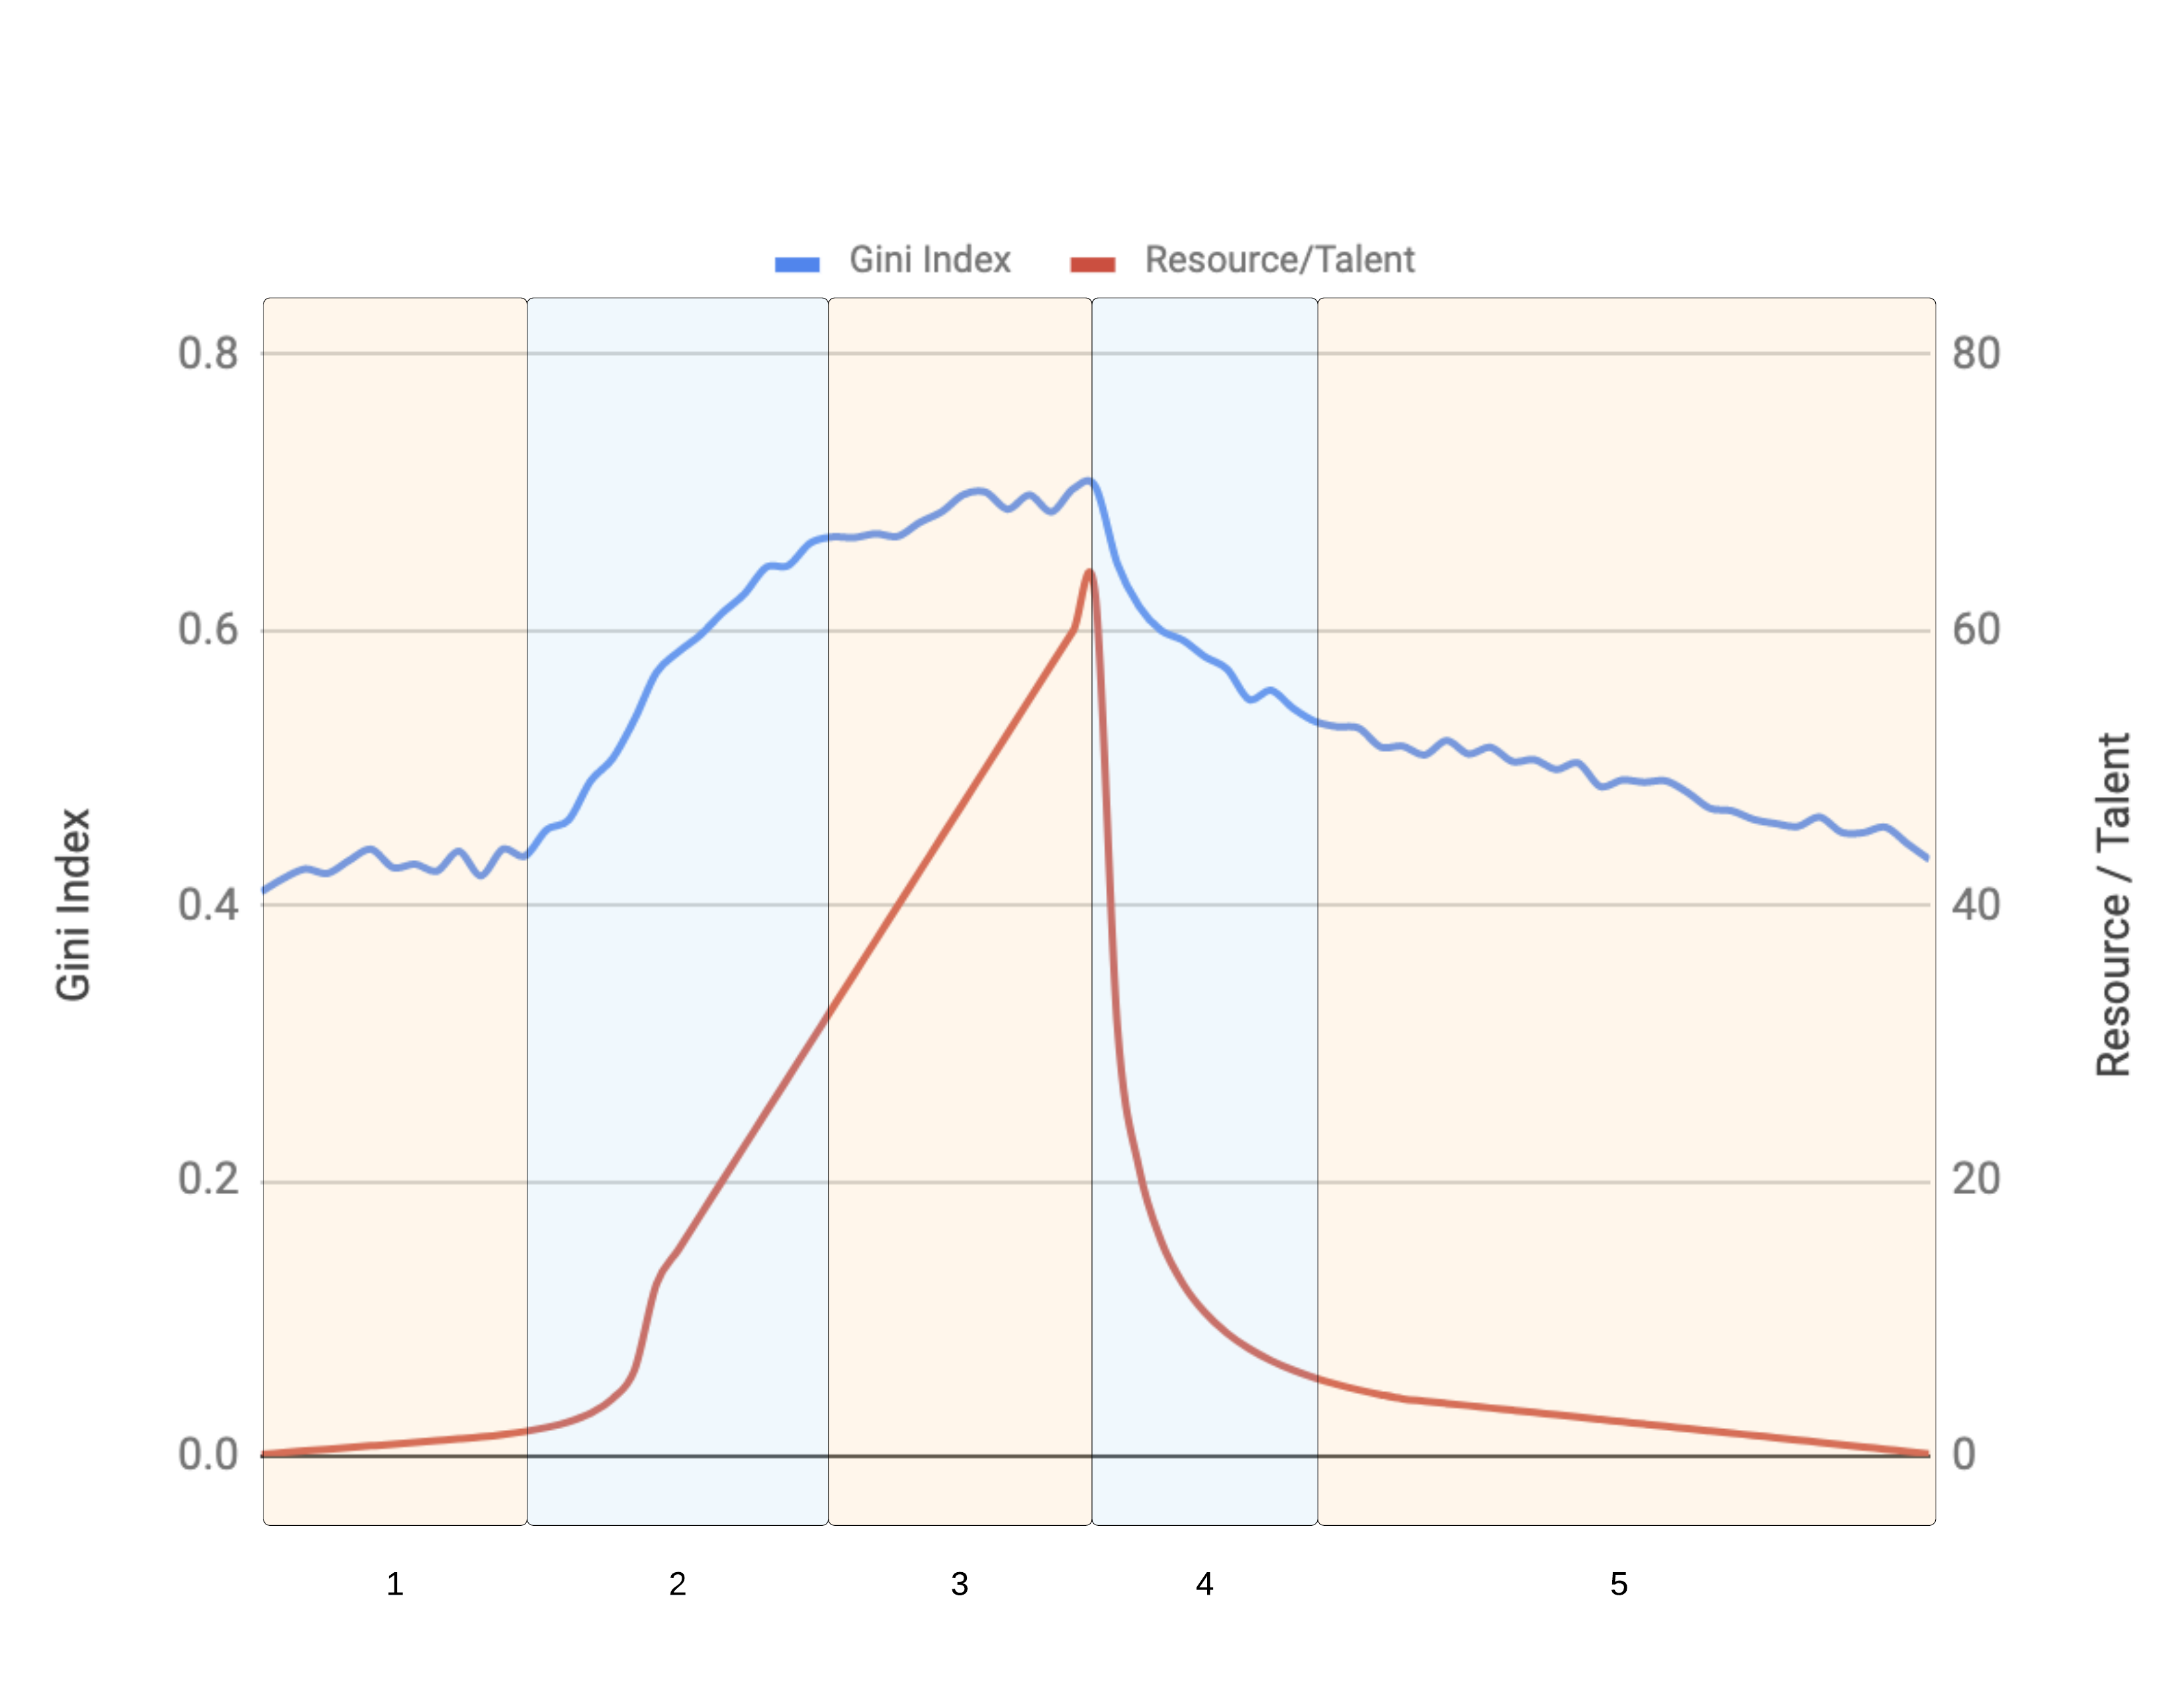
\includegraphics[scale=0.4]{Wealthy_Modell_ex_1.png}
	\end{center}
\end{figure}

The curve of Gini index can be depart to five phases.
\begin{itemize}
	\item 1st phases: 1-13\\
	During this phase, The total resource in the world is very limited, The mainly source of grains is from rebirth. Thus, the Gini index keeps in a low degree and increases slowly.
	\item 2nd phases: 14-26\\
	The Gini index has a remarkable growth in this phase with the total resource increase.
	\item 3rd phases: 27-39\\
	When the resource grow to a high level, the Gini index will not continue increasing, it will remain at a relatively stable level. This might be the most darkness time of the virtual world. There are sufficient resource but an extreme gap between the poor and the rich.
	\item 4th phases: 40-46\\
	This is an exciting result. It shows that even a little improvment of people's ability will obviously eliminate the wealthy gap.
	\item 5th phases: 47-77\\
	When the $Talent$ increase to a threshold, we notice that the Gini index will slowly reduce. Eventually, The Gini index will back to the same level as the very beginning.
\end{itemize}
\subsection{Results of Extended Model}
All three extensions are tested in rich, normal, poor circumstances.  In poor circumstance,  people die and reborn every clock so the performance of system is quite similar as original model no matter what extension added in system. Without inheritance, all simulate results in poor circumstance are same as below: 
\begin{center}
	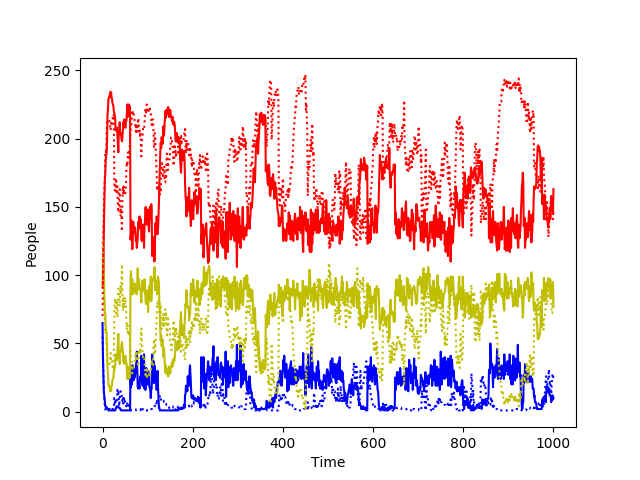
\includegraphics[scale=0.5]{poor.png}
\end{center}
We find that our three extensions don't impact the final wealth distribution under most situations. However, there is a huge difference during the evolution such as evolution speed and fluctuation. Here we will discuss the results from extensions to answer the questions addressed above. 
\subsubsection{Heritage Inheritance}
The result of extension prove our assumption that the heritage inheritance will speed up evolution of wealth distribution. The experiment result also shows that the movement between class of people become less (almost 0) after we add inheritance mechanism. Finally, the Gini-index arrive 0.8 which means there are a huge gap between rich and poor in this world.
\begin{figure*}[h]
	\centering
	\begin{subfigure}[t]{0.5\textwidth}
		\centering
		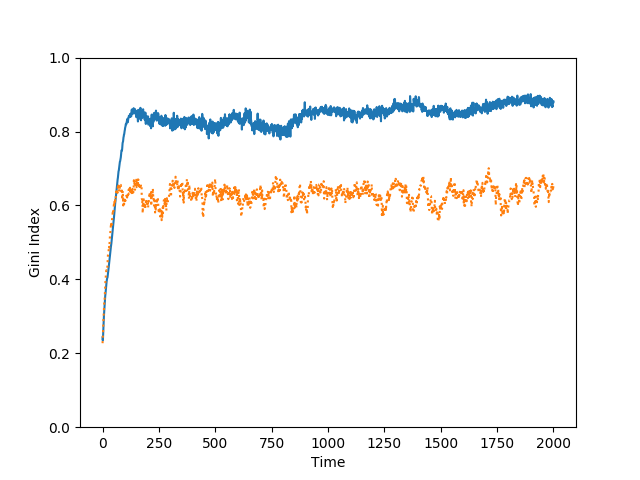
\includegraphics[scale=0.5]{inheritance_gini.png}
	\end{subfigure}%
	~ 
	\begin{subfigure}[t]{0.5\textwidth}
		\centering
		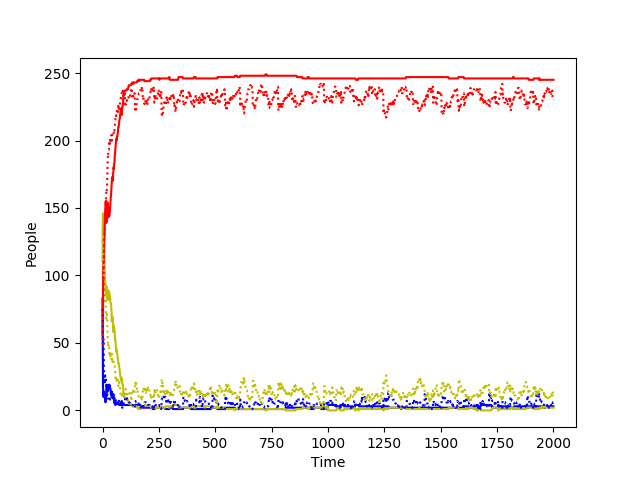
\includegraphics[scale=0.5]{inheritance_classes.png}
	\end{subfigure}
\end{figure*}

\newpage
\subsubsection{Season}
We define the 100 clocks as 1 year and divide it into 2 parts, summer and winter. 
\begin{figure}[H]
	\begin{center}
		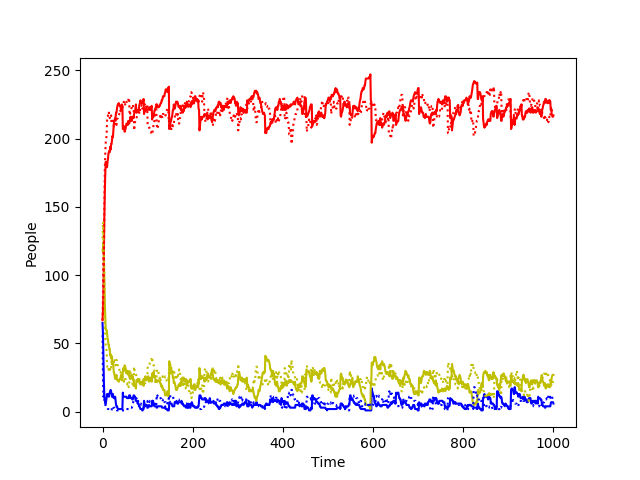
\includegraphics[scale= 0.6]{season.png}
	\end{center}
\end{figure}

It could be found that there are more fluctuations in new model. We find that season is a complex factor to impact the wealth distribution. In rich or middle circumstance, there is no significant difference. In poor circumstance, large number of poor people could not survive from winter.\\

Finally, we get the conclusion of relationship between season and wealth distribution, which is that season may put pressure on everyone's life. However, the rich can get over it with bench of savings while the poor may not be able to survive if the situation is too severe.

\subsubsection{Reclamation}
We implement reclamation function by replacing grains of two random lands. Based on result we get from simulator, we find that there is redistribution process every time reclamation happens. It relatively slows down the evolution speed.
\begin{figure}[H]
	\begin{center}
		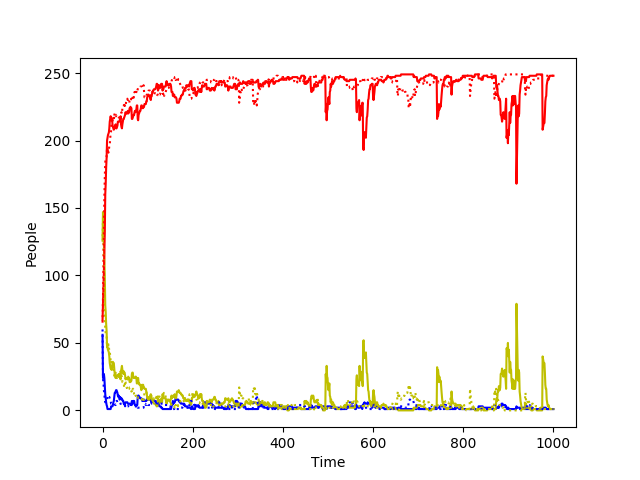
\includegraphics[scale= 0.6]{reclamation.png}
	\end{center}
\end{figure}

If we reduce the vision of people and increase the frequency of reclamation, the result would be more obvious. The more interesting thing is that the movement of people between poor and middle become more frequent after a while. In this situation the Gini-Index value also reduced.
\begin{figure*}[h]
	\centering
	\begin{subfigure}[t]{0.5\textwidth}
		\centering
		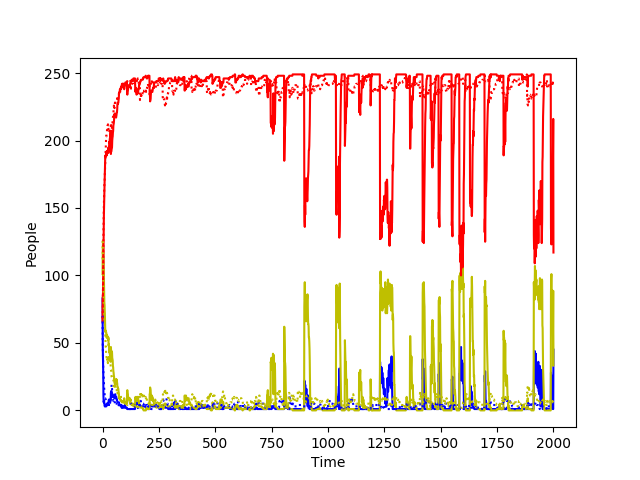
\includegraphics[scale=0.5]{final.png}
	\end{subfigure}%
	~ 
	\begin{subfigure}[t]{0.5\textwidth}
		\centering
		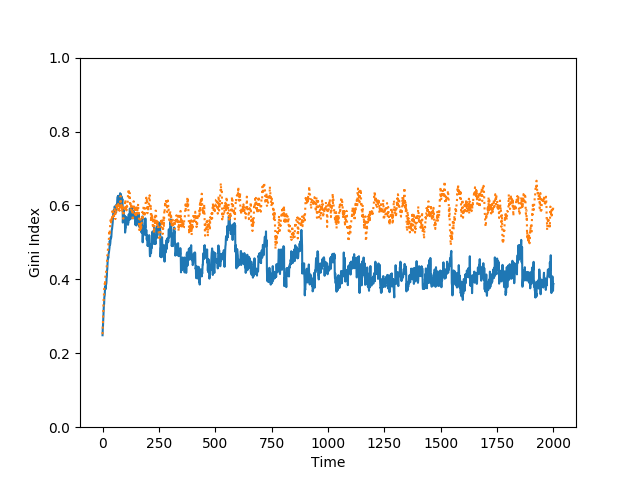
\includegraphics[scale=0.5]{gini_index.png}
	\end{subfigure}
\end{figure*}
\section*{Appendix}
In our group, Rui Zhao focuses on implementing the replicated model based on the original NetLogo model. Weikai Zeng implements the extensions with the base of replicated model. Yang Zhang concentrates on writing the reports.\\

Our statistic data stored on the drive. The link shows here: \url{https://drive.google.com/open?id=1Qio2P0ql1nWkcCwRySZ5nTG3h6K63MwPTOnkG8sOdPI}

During implementing the whole wealth distribution system, we met two challenges and wish to overcome it in the future.
\begin{itemize}
	\item Firstly, we actually didn't find out a possible way to prevent or mitigate the wealth distribution gap between the poor and the rich. 
	\item Secondly, we would have wanted to implement the loan system as extension. However, we find
	that it's also a very complex system as we can't track every single person in our system.
\end{itemize} 


\end{document}